% !TeX spellcheck = en_US

\chapter{Foundations and Related Work}
\label{chap:ch2}
\label{chap:foundation}

In the exploration of chatbot technology and its applications, this section delves into foundational aspects and related work that form the basis of effective chatbot development. 
The foundations include concepts such as smart homes, chatbot types, and building blocks, providing insights into the underlying principles and methodologies. 
As the foundation is established, the discussion extends to related work, examining existing literature on chatbots in smart homes and their applications in complex scenarios. 
By understanding these foundational elements and existing research, the subsequent sections aim to contribute novel insights and advancements in the field of chatbot development.

\section{Foundations}
\label{sec:foundation}
In this subsection, the focus are the specific foundations that are crucial for the development of chatbots.
Including key elements for this thesis such as a definition for a Smart Home and Natural Language Understanding which enables chatbots to understand a users input message.
Other elements such as a general architecture and typical building blocks for chatbots are also presented.

\subsection*{Smart Home} 
A smart home devices main aspect is that its original functionality is augmented through network capabilities \cite{schiefer_smart_2015,balakrishnan_smart_2018} and should enhance especially comfort\cite{matsui_information_2018, balakrishnan_smart_2018} but also security\cite{balakrishnan_smart_2018} or energy efficiency\cite{matsui_information_2018, balakrishnan_smart_2018} for example. 
Therefore a smart home consists of such devices and provides additional infrastructure like an app to control the devices. 
These infrastructures often allow automation of the devices.
Since its functionality is based on connected devices and often sensors it is often named in the context of the Internet of Things (IoT) \cite{atzori_internet_2010}. 

\subsection*{Chatbot Types and Classifications}
% lehmann
Based on Lehmann \cite{lehmann_chatbot-guide_2021} there are three main types of chatbots: decision-tree-based, keyword-based, and advanced context-aware bots. 
Decision-tree-based bots follow a predefined flowchart in response to user queries, often identified by menus and buttons. 
Keyword-based bots recognize specific keywords, making decisions and providing responses based on internal knowledge. 
Advanced context-aware virtual assistants engage in free-flowing conversations, learning from interactions and offering versatile responses.

% adamopoulou
Additionally, according to Adamopoulou and Moussiades\cite{adamopoulou_overview_2020} chatbots can be classified based on their \textbf{knowledge domain}, with open domain bots discussing general topics and closed domain bots focusing on specific knowledge domains. 
In terms of \textbf{service}, interpersonal chatbots act as information intermediaries, offering communication services like restaurant or flight booking. 
Intrapersonal chatbots, existing within the user's personal domain, function as companions, understanding users like humans. 
Inter-agent chatbots, omnipresent in nature, facilitate inter-chatbot communication. 
\textbf{Goal-based} classification includes informative chatbots providing stored information, chat-based bots conversing like humans, and task-based bots performing specific functions intelligently. 
\textbf{Input processing and response generation} methods vary, from rule-based models relying on predefined rules to retrieval-based models using APIs, and generative models employing machine learning techniques. 
\textbf{Human-aided} chatbots incorporate human computation for flexibility and robustness.
The \textbf{build method} distinguishes between open-source platforms allowing intervention and closed platforms acting as black boxes but providing immediate access to advanced technologies, often found in large companies.

\subsection*{Chatbot Building Blocks}
In this subsection building blocks and architectural insights that can be identified in different literature are collected and explained. 
It is mostly based on Lehmann \cite{lehmann_chatbot-guide_2021} and \cite{adamopoulou_overview_2020} if not mentioned otherwise.

\subsubsection{Natural Language Understanding (NLU) and Machine Learning}
NLU, a subset of Natural Language Processing (NLP), is essential for chatbots.
It involves training algorithms to understand and process natural language, bridging the gap between human language and artificial intelligence. 
NLU is critical for successful chatbot operation, enabling the machine to comprehend user intents and contexts.

Machine learning and NLP also play roles in the evolution of virtual assistants. 
Machine learning algorithms, based on training data, build statistical models and autonomously improve over time.
NLP focuses on processing and understanding natural language, incorporating elements from computer science, AI, linguistics, and data mining. 
These technologies empower chatbots to interpret complex human language, allowing for more sophisticated and context-aware interactions.

\subsubsection{Intents}
Chatbots operate with three key components – Utterances, Intents, and Entities. Intents represent different user intentions that a chatbot anticipates, each consisting of various utterances (training phrases) and one or more responses. Utterances are potential user expressions or example questions, and entities are real-world objects mentioned in a sentence. This structure facilitates the interpretation of natural language, enabling chatbots to recognize user intents and associated entities for effective communication.

Chatbots are built on different intents, each with various utterances and responses. 
The training involves teaching the bot to recognize user intents based on a set of training phrases. 
A Natural Language Processing Engine interprets natural language, transforming it into structured language, and identifies entities within sentences to enhance contextual understanding.

There are also narrow work that regard intent-based chatbots as a separate species \cite{luo_critical_2022}. 
These then typically deal with the technique used to generate responses to ultimately categorize the chatbots.

\subsubsection{Knowledge Bases}
Knowledge bases serve as a crucial component for chatbots, providing them with the necessary information to respond intelligently to user queries. 
These databases store domain-specific data, facts, and contextual information that enable chatbots to understand and address user requests accurately.

\subsubsection{General Chatbot Architecture}
In general, the chatbot architecture by Adamopoulou and Moussiades\cite{adamopoulou_overview_2020} which can be seen in \cref{fig:chatbot-architecture-general} consists of components such as the Language Understanding Component, which interprets user requests and identifies intentions and associated information, and the Dialogue Management Component, which keeps track of the conversation context, processes clarifications, and asks follow-up questions. After understanding the user's request, the chatbot executes actions or retrieves data from its Knowledge Base or external resources, and the Response Generation Component generates natural language responses based on the intent and context information.


\iffalse
\subsubsection{A chatbot taxonomy}
\begin{figure}[h]
\centering
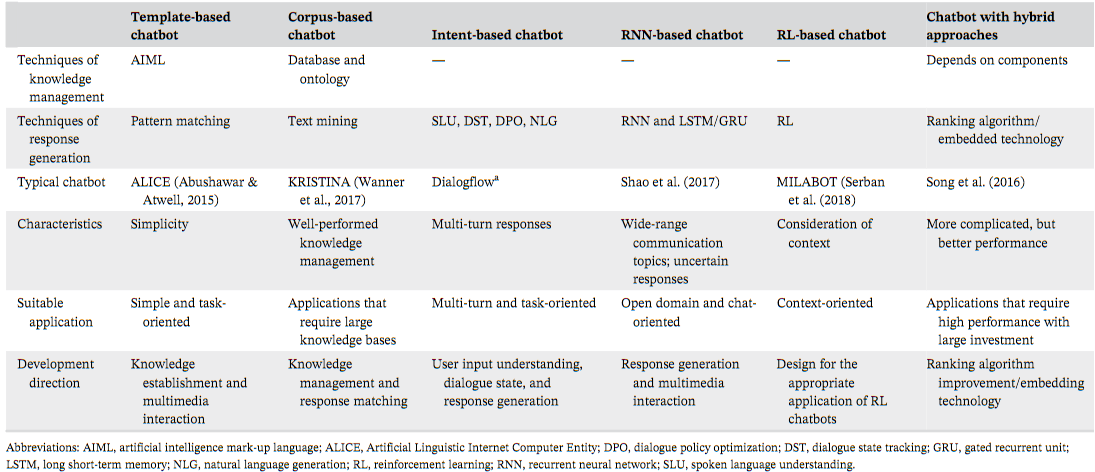
\includegraphics[width=0.98\textwidth]{graphics/chatbot-taxonomy-raymond.png}
\caption{An example taxonomy of chatbots \\Source: Luo et al. \cite{luo_critical_2022}}
\label{fig:chatbot-taxonomy}
\end{figure}
\newpage
\fi


\subsection*{Prototype and Iterative Development}

This subsection is based on Sommerville \cite{sommerville_software_2011} according to who "iterative development of the prototype is essential".
The process for developing a prototype is shown in \cref{fig:prototype-process} and summed up consists of planning, developing and evaluating.
Another iterative process is the extreme programming release cycle which is shown in \cref{fig:extreme-prog-cycle} and consists of user stories that are selected and developed throughout one cycle.
Based on this concepts and needs for our chatbot prototype we built the iterative development cycle that is shown in \cref{fig:iterative-design} which could be seen as a combination of the both processes presented in this subsection.
It is useful to start projects like this thesis with a prototype with thought out case \cite{lehmann_chatbot-guide_2021}.

\begin{figure}[t]
\centering
\captionsetup{justification=centering}
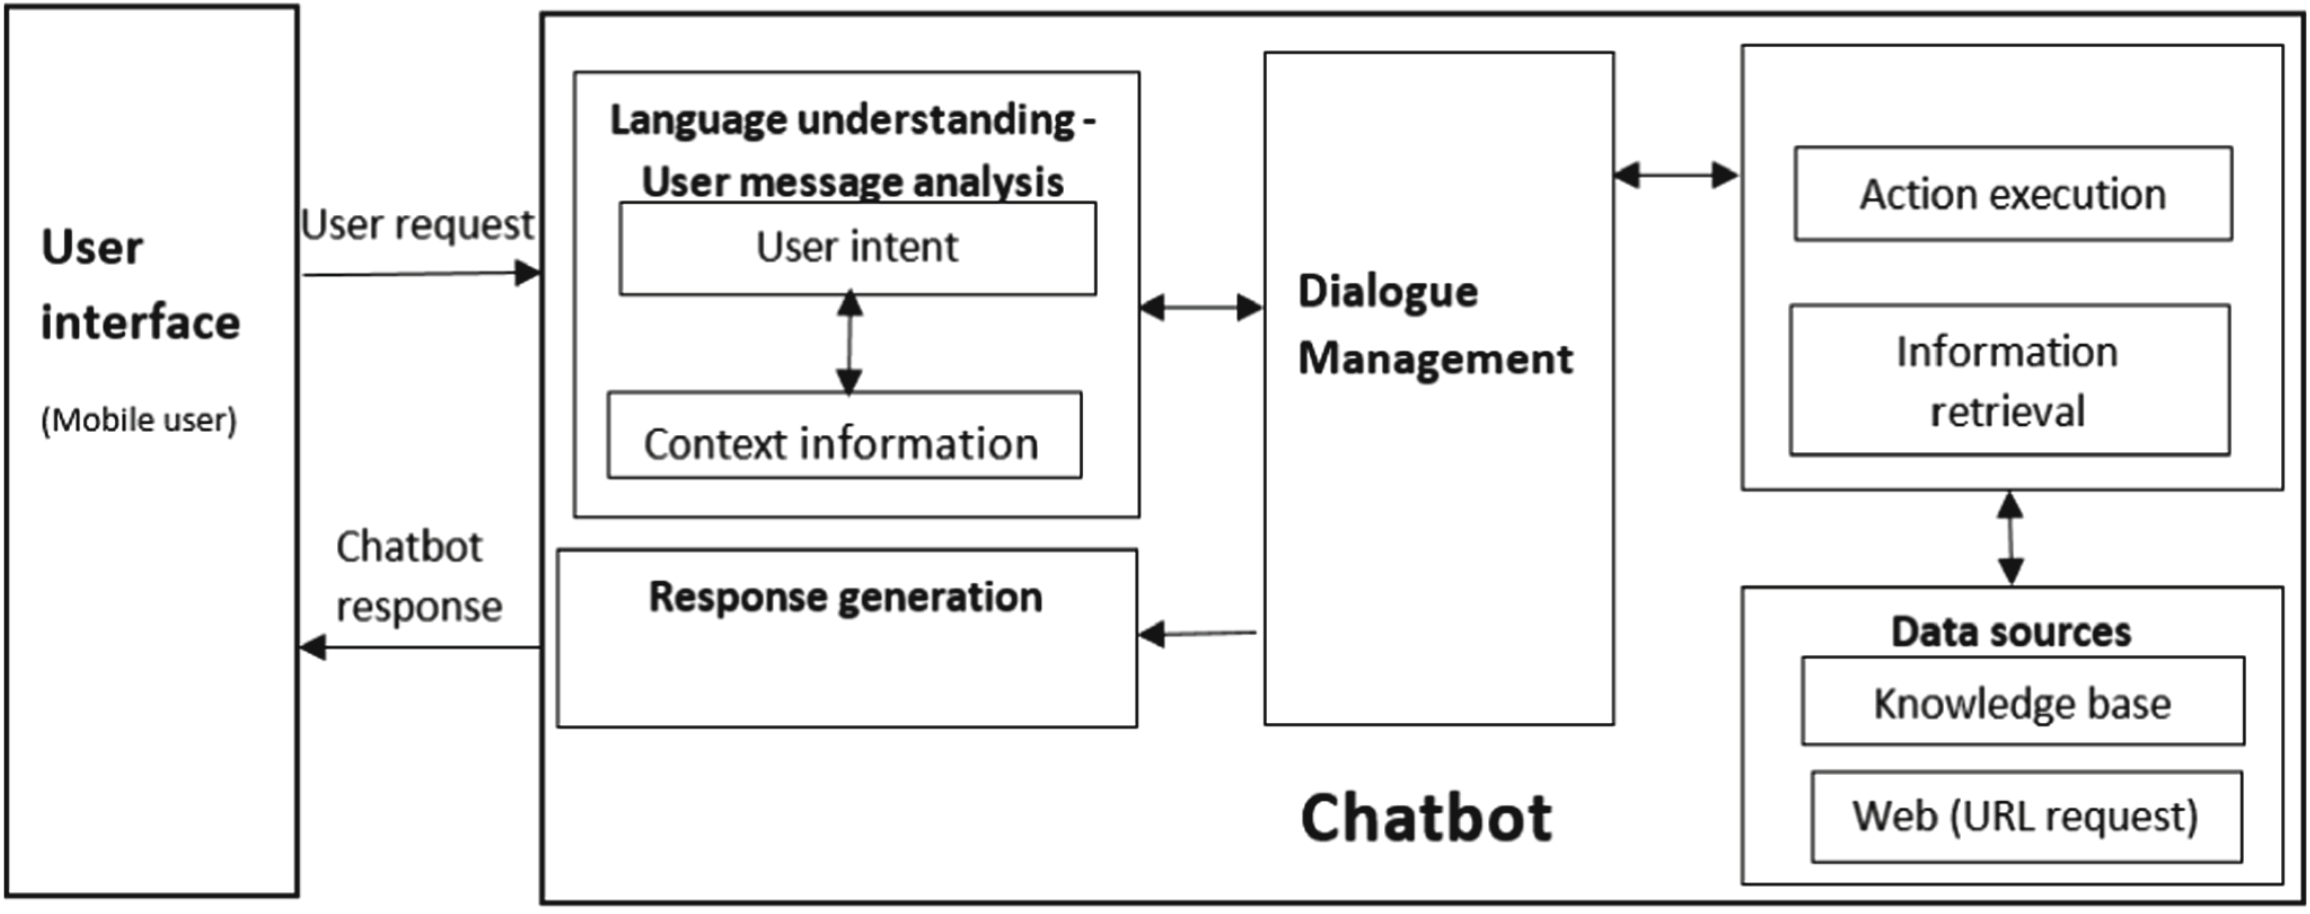
\includegraphics[width=0.98\textwidth]{graphics/chatbot-architecture-general.png}
\caption{An example architecture of chatbots in general \\Source: Adamopoulou and Moussiades \cite{adamopoulou_overview_2020}}
\label{fig:chatbot-architecture-general}
\end{figure}

\begin{figure}[h]
\centering
  \begin{subfigure}{.7\textwidth}
    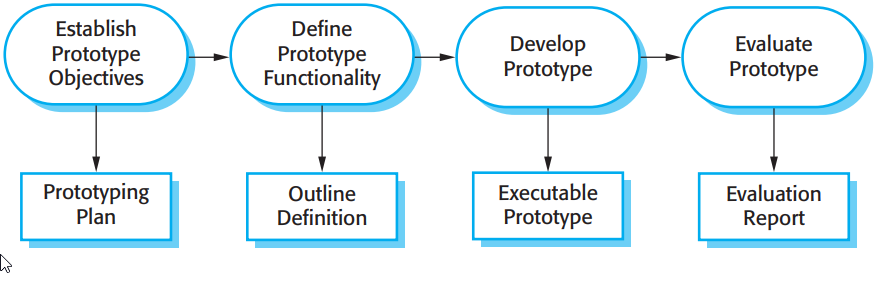
\includegraphics[width=\textwidth]{graphics/prototype-dev.png}
    \caption{Prototype development process}
    \label{fig:prototype-process}
  \end{subfigure} \hfill
  \begin{subfigure}{.63\textwidth}
    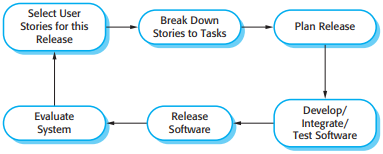
\includegraphics[width=\textwidth]{graphics/extreme-programming-release-cycle.png}
    \caption{Extreme programming release cycle}
    \label{fig:extreme-prog-cycle}
    \end{subfigure}
  \caption{Visualized development processes \\ Source: Sommerville \cite{sommerville_software_2011}}
  \label{fig:dev-processes}
\end{figure}

\newpage
\section{Related work}
In addition to discussing about foundations, you need to discuss about why the problem you are tackling has been insufficiently solved before. To do so, you need to mention related work and discuss what is the difference between your work and those related works.
This section presents literature that is related to this thesis.
While chatbots are ever known to be used in areas like customer service it is interesting to see work on how chatbots are used in smart homes or for complex scenarios like managing containerized networks.
Some literature has the nice side effect that it also presents the architecture of the developed system and can inspire the architecture of the chatbot that should be developed in this thesis.

\subsection*{Chatbots for Smart Homes}
Various literature exists that contains some kind of chatbot in the context of Smart Homes.
Most of these chatbots perform the same task as nowadays common Voice assistants as for example the Google Assistant\footnote{\href{https://assistant.google.com/}{assistant.google.com}} which is capable of understanding written request but also transforming speech into written requests which also includes managing smart devices added to Google Home\footnote{\href{https://home.google.com/intl/de_de/the-latest/}{home.google.com}}, an app for managing a smart home.

Baby et al.\cite{baby_home_2017} presented an approach for a chatbot that can control multiple smart devices in a smart home.
The developed prototype is capable of answering simple questions that regard the devices or change variables of the devices.
It is able to answer questions like "What is the temperature in room 1" or "Set the temperature to 19 degrees celsius".
The architecture includes multiple building blocks that were explained in \cref{sec:foundation}: An NLP Pipeline which in the end identifies the intent of a message and matches an action to.
The pipeline can be seen in \cref{fig:chatbot-pipeline-baby}
The intents and pipeline of this chatbot could inspire the inital iteration of our prototype. 
\begin{figure}[h]
\centering
%\captionsetup{justification=centering}
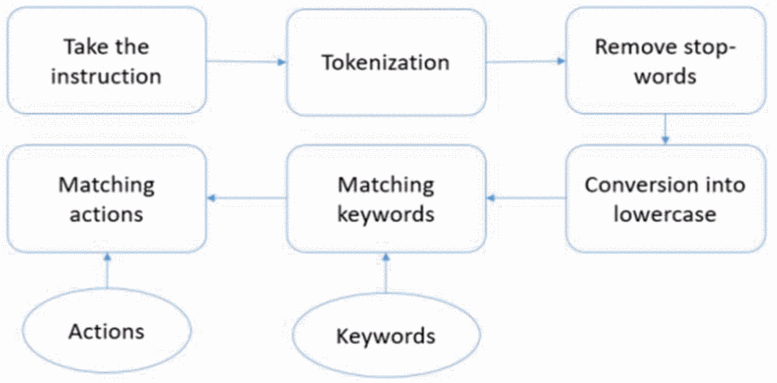
\includegraphics[width=0.66\textwidth]{graphics/baby2017chatbot.png}
\caption{A simple NLP pipeline for a chatbot \\Source: Baby et al. \cite{baby_home_2017}}
\label{fig:chatbot-pipeline-baby}
\end{figure}

Another work developed and connected a chatbot to the facebook (today called meta) messenger for controling smart home devices fans and lights but also gas leakage detection or humidity monitoring \cite{ahmed_smart_2020}.
Intents are not clearly defined or at least not stated but it seems to be a simple decision-tree-based chatbot.
This is probably due to focus of the work laying more in the systems architecture and a limited amount of intents.

A different work explored the area of collaboratively teaching where a focus was set on mitigate malicious activities \cite{chkroun_safe_2021}.
The presented chatbot called Safebot is intended as an extension to smart home assistants and is able to communicate when it does not know the answer the a request and can be taught afterwards.
Also, users could notify the bot that an response was not appropriate resulting in also teaching it.
The learning is purely based on natural languages in contrast to chatbots that for example use knowledge bases with structured data.

\subsection*{Chatbots for complex Scenarios}
Various chatbots for many different use cases exist. 
As the intention of this work is to test how far a chatbot can go in answering complex queries to a smart home the question aligns if approaches exist for answering (complex) questions in a closed domain based on available data.
An example for this is the work of Ait-Mlouk and Jiang \cite{ait-mlouk_kbot_2020} which approached to develop a knowledge graph based chatbot that can find information in linked data through NLU.
The researches in this work address challenges like understanding many different queries (and intents) and making the use of multiple languages and knowledge bases available.
The system developed is able to be extended with new domains.
The architecture of it can be seen in \cref{fig:kbot}.
While it is too complex to explain in detail, it processes queries into intents and entities (through Named Entity Recognition) which in combination make it possible to retrieve information from connected knowledge bases by transforming it into queries and selects a response based on a knowledge graph.

\begin{figure}[h]
\centering
%\captionsetup{justification=centering}
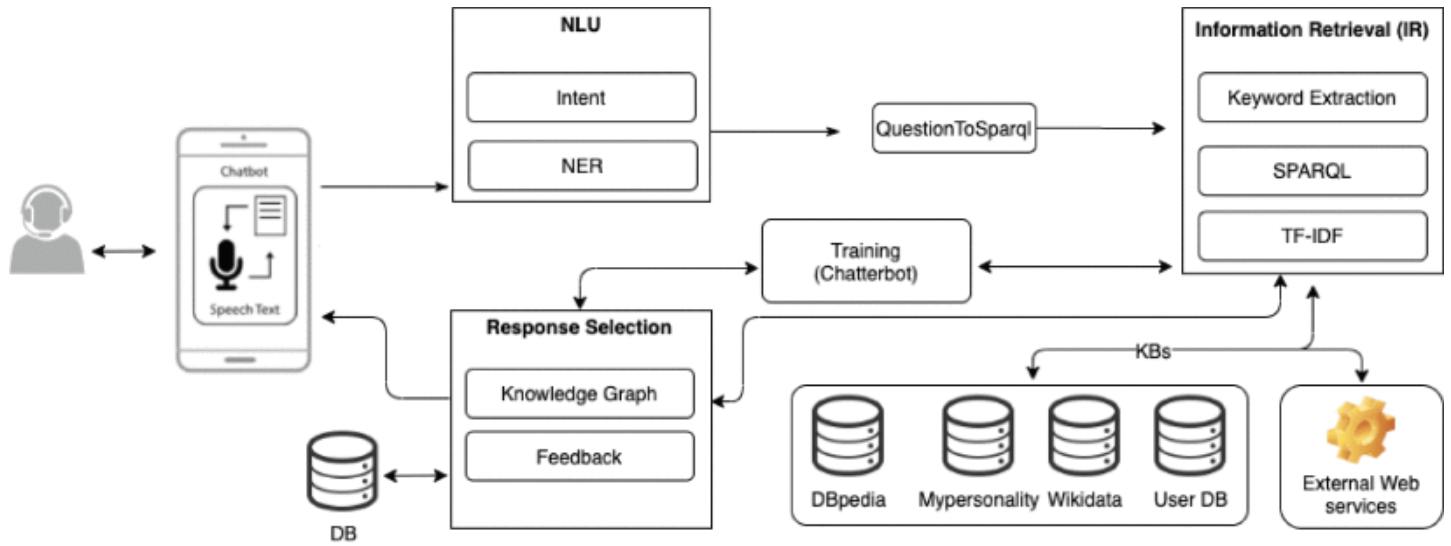
\includegraphics[width=0.94\textwidth]{graphics/KBot-architecture.png}
\caption{Detailed Architecture of KBot \\Source: Ait-Mlouk and Jiang \cite{ait-mlouk_kbot_2020}}
\label{fig:kbot}
\end{figure}

Another research presented a chatbot that can create and manage a containerized network, thus acting as a workflow manager \cite{jasinski_chatbot-based_2023}.
It enables less human involvement by computing requirements written by users.
This leads to a decreasing need for users to have extensive knowledge of the underlying tools to be able to setup such networks and also makes the management of them easier in general.
This can be mapped to this thesis where one aim is to enable even users with less technology knowledge to analyze complex scenarios in their smart home and to make the analysis of those easier in general.

A different work \cite{carlander-reuterfelt_jaicob_2020} approached to develop a chatbot that helps to gain knowledge about Data Science and Machine Learning.
The architecture includes information retrieval from a knowledge base, parsing the received document and answering a query based on the search in the knowledge base.
It also includes a "Small Talk Module" which improves users satisfaction with the system and increase the overall interest in chatting with it.

%noch etwas Fülltext
%\blinddocument
